% !TEX root = ../Thesis.tex
%\documentclass{article}
%\usepackage{graphicx}
%\usepackage{xcolor}
%\usepackage[utf8]{inputenc}
%\usepackage{siunitx}
%\usepackage{hyperref}
%\newcommand{\imsize}{\linewidth}
%\begin{document}
\pagestyle{empty}
\hfill
\vfill
\begin{figure}[h]
	\noindent\makebox[\textwidth]{%
		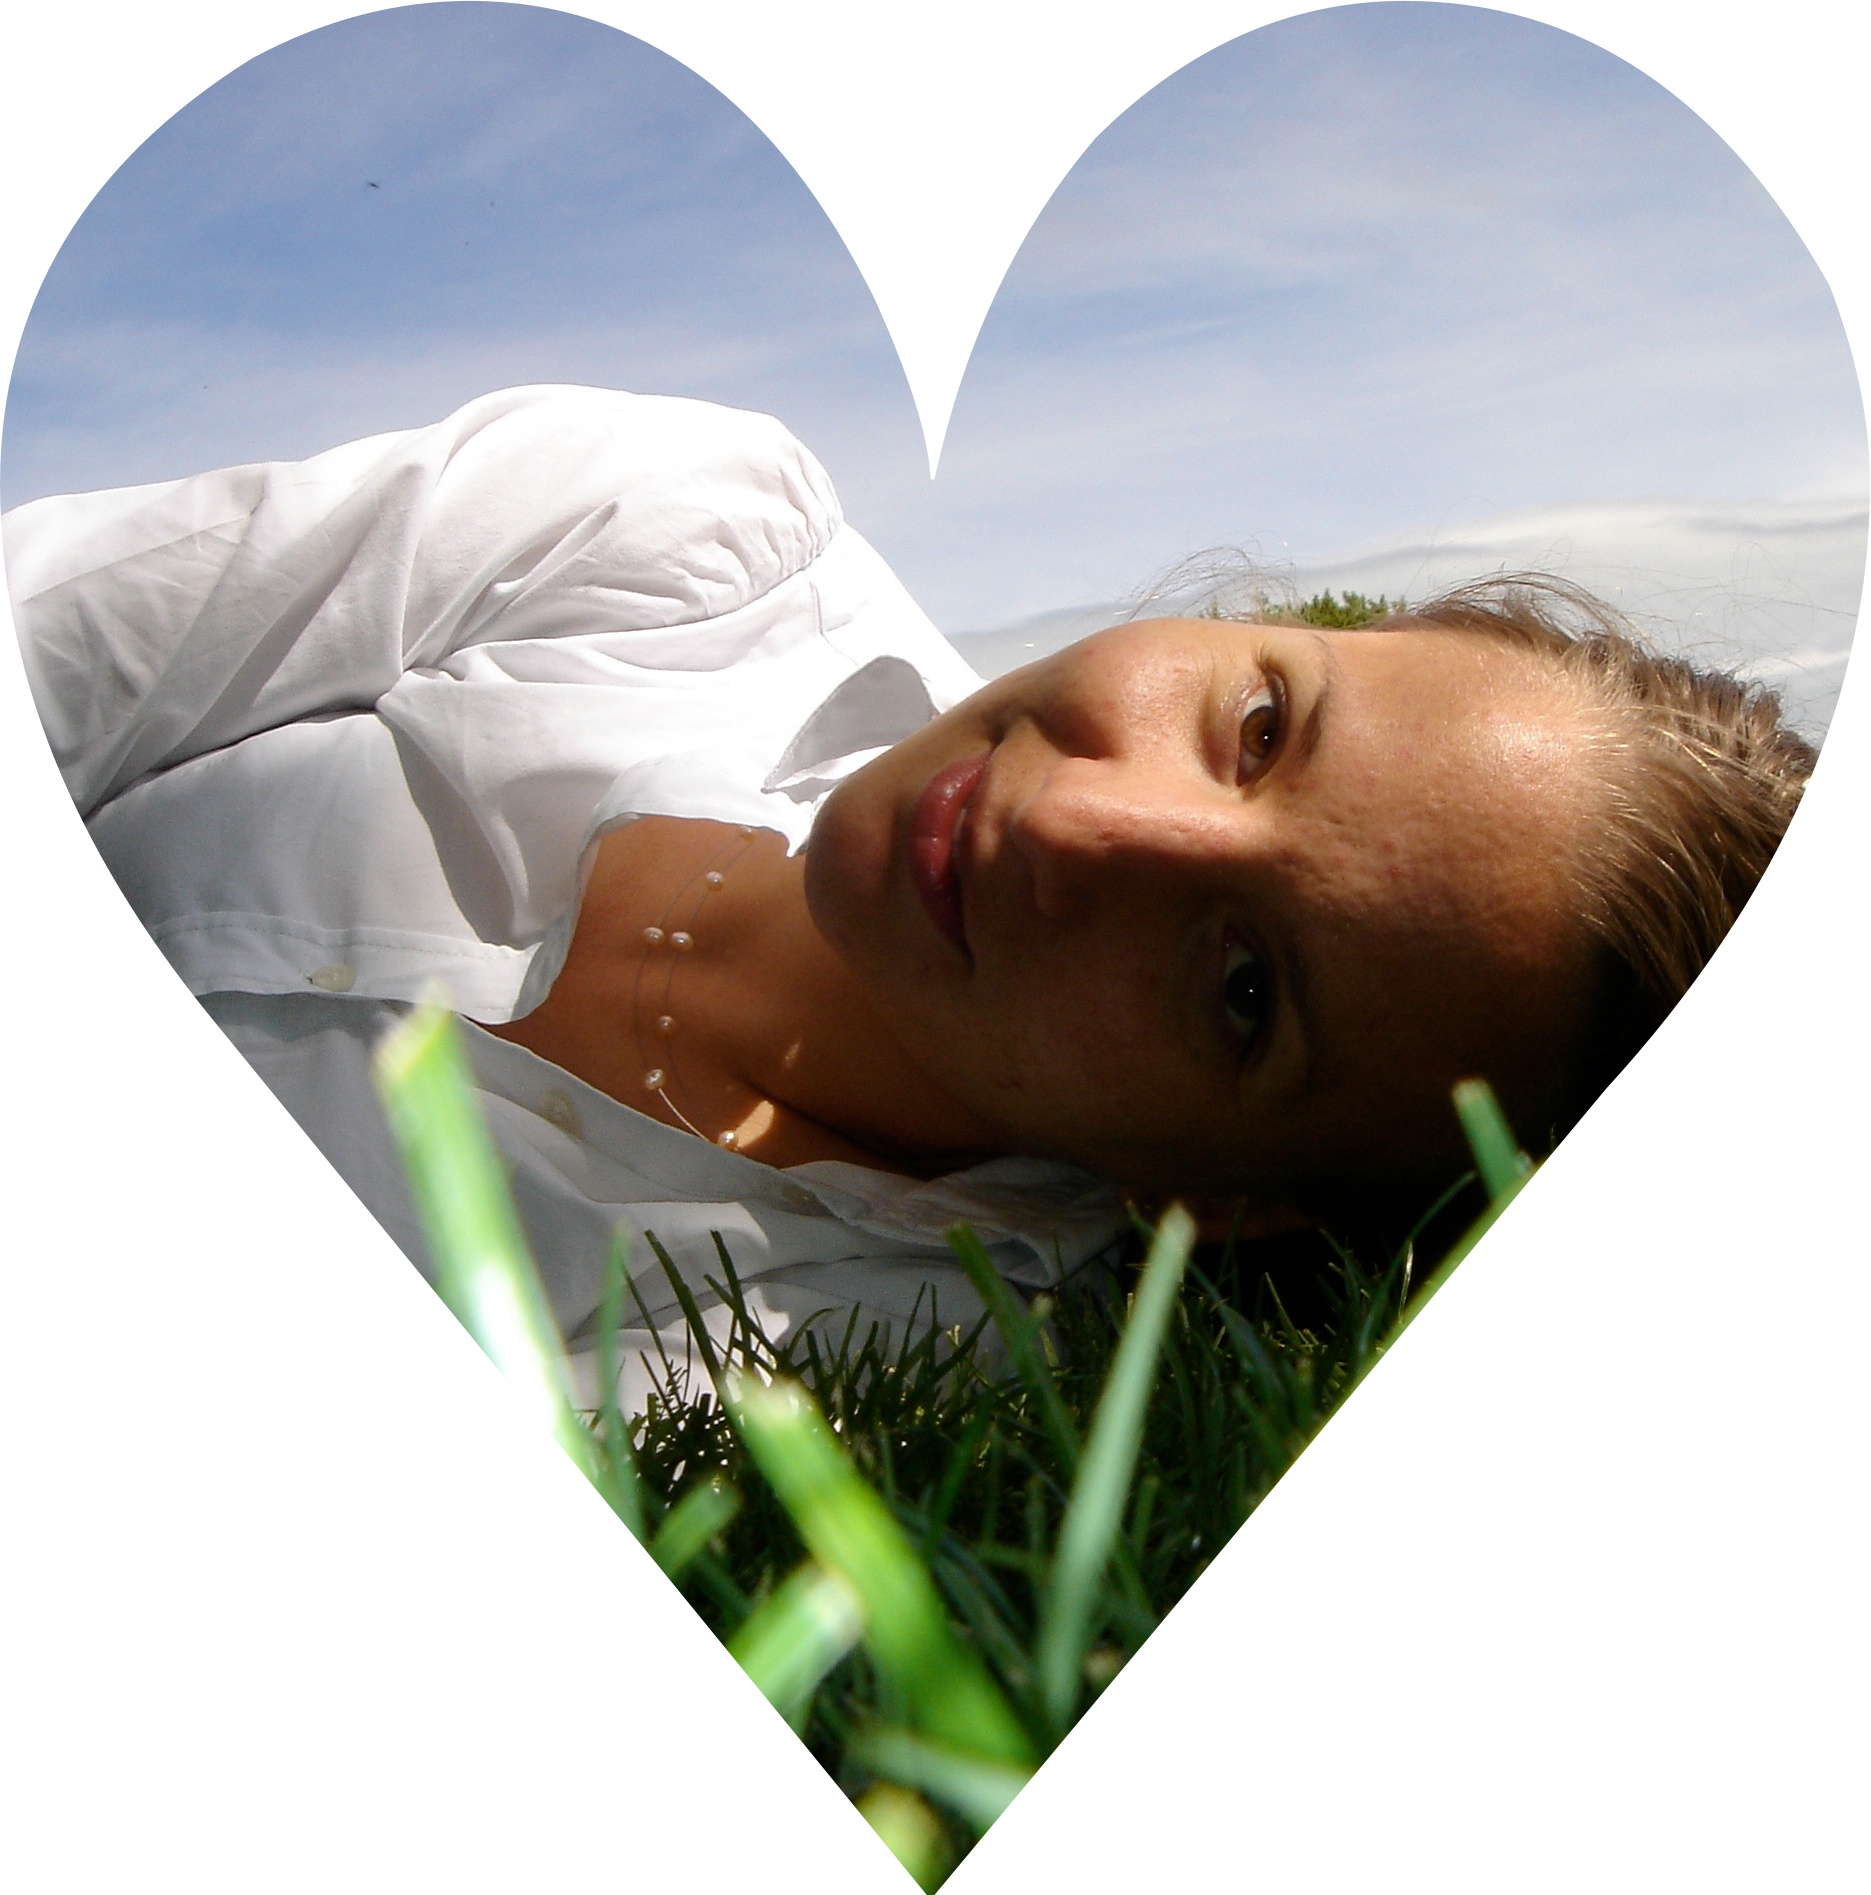
\includegraphics[width=\imsize]{FrontBackmatter/nina-gurten}%
	}%
	\caption{\href{http://maps.google.com/maps?q=46.918577,7.440087&num=1&t=h&sll=46.9185,7.4401&sspn=0.015244,0.032015&hl=en&ie=UTF8&ll=46.918672,7.440126&spn=0.005753,0.012821&z=17}{Für Nina: +46\degree 55'6.60", +7\degree 26'24.36"}}%
	\label{fig:<3}%
\end{figure}%
\vfill
Nina, von diesem Foto über meinen zwei Bildschirmen hast du mich die letzten Jahre immer wieder voller Liebe angeschaut.

Für das Glück, welches du mir schenkst, die Unterstützung, die du mir gibts und die Liebe, die ich von dir bekomme, bin ich dir unglaublich dankbar.

Du bist die Beste!
\newline

\centering
{\color{red}$\heartsuit$}
\vfill
%\end{document}